\chapter{Introdução}

\noindent 

	A simulação computacional é uma ferramenta de emprego crescente, que não se limita ao domínio da engenharia, sendo ampliada para aplicações em diversos setores da ciência contemporânea. Já é possível modelar simulações para campos aerodinâmicos, biológicos, meteorológicos e até financeiros. Tal recurso é extremamente útil para a compreensão de fenômenos complexos, de variadas amplitudes no domínio temporal e para a economia de recursos e tempo em projetos de engenharia.
	
	A engenharia moderna possui como alguns dos principais desafios a otimização de sistemas já existentes e a modelagem de novos sistemas com excelentes rendimentos mecânico e térmico. Ainda, essas melhorias devem ocorrer em paralelo com um baixo custo associado de forma a manter a competitividade no mercado. Antes do avanço tecnológico das últimas décadas, a resolução de problemas físicos demandava um grande esforço e custo em função da necessidade de reprodução material, mas esse método pôde ser substituido com teorias bem trabalhadas e fundamentadas em experimentações passadas, modelagens físicas e matemáticas aplicadas em uma resolução numérica-computacional.
	
	Dentre os vários ramos da engenharia, a mecânica dos fluidos é um grande exemplo de aplicação dos métodos supracitados. Tópicos como turbulência, troca de calor e interação fluido-estrutura são trabalhados de forma extensiva na pesquisa, e têm apresentado resultados muito coerentes com aqueles observados pelo método empírico. 
	
	Este trabalho objetiva a execução de análises matemáticas e discretizações numéricas para os transportes por difusão e advecção para os casos unidimensional e bidimensional, sob a metodologia explícita e implícita. Tais mecanismos são observados na transferência de energia térmica em escoamentos laminares, de transição e turbulentos em proporções particulares para cada caso. Os diferentes tratamentos do termo temporal são trabalhados de forma conjunta para a comparação da relação entre custo computacional e estabilidade numérica de ambos. A partir da modelagem numérica das equações associadas, se produz um código, ou modelo computacional, que resolve numericamente o problema a partir de uma condição inicial e condições de contorno conhecidas, finalmente comparando a solução numérica com a analítica.
	
	%Por fim, escoamentos heterogêneos, também tratados neste trabalho, são de grande importância para a mecânica dos fluidos devido à sua extensa ocorrência na prática da engenharia mecânica. O estudo de tais escoamentos possibilita uma modelagem de carregamento de particulado com o fluido durante a extração de petróleo ou a troca de calor em um líquido em transição de fase, por exemplo.
	
\newpage
	

 \section{Metodologia}
 % --------------------------------------------------------------------------

\noindent

	A metodologia proposta para o presente trabalho de iniciação científica se baseia
na definição de problemas, estudando primeiramente os casos particulares, e uma vez
compreendida a natureza do conteúdo, seguindo para problemas mais gerais e complexos.

	Inicialmente verifica-se na literatura as dinâmicas envolvidas nos mecanismos propostos para este estudo. A partir das relações obtidas nessa revisão, elabora-se uma discretização a partir de métodos numéricos e realiza-se a implementação dos mesmos em um código computacional. As rotinas são confeccionadas na linguagem de programação Fortran, para familiarização do aluno com a linguagem base dos códigos do Laboratório de Mecânica dos Fluidos Computacional (MFLab) da Faculdade de Engenharia Mecânica (FEMEC) da Universidade Federal de Uberlândia.
 

\subsection{Difusão}

\noindent

	A difusão é um mecanismo de transporte que possui diferentes definições nos campos da química, biologia e física. Especificamente para o caso de transferência de calor, a difusão é bem definida matematicamente por uma equação diferencial parcial (EDP), que envolve uma derivada parcial de primeira ordem no domínio temporal e uma derivada parcial de segunda ordem no domínio espacial. Os termos são relacionados, através de uma constante (difusividade), à um termo fonte, resultante da diferença desses elementos, como indicado na Eq. (\ref{Difusaoone}).
	
\begin{align}
 \label{Difusaoone}
 f(x,y,z,t) = \dfrac{\partial \phi}{\partial t} - \alpha \nabla^2 \phi
\end{align}

	Assim, para o caso unidimensional, obtém-se a relação dada pela Eq.(\ref{Difuni}).
	
\begin{align}
 \label{Difuni}
 f(x,t) = \dfrac{\partial \phi}{\partial t} - \alpha \left(\dfrac{\partial^2 \phi}{\partial x^2}\right)
\end{align}

	E para o caso bidimensional, obtém-se a relação dada pela Eq.(\ref{Difbi}).
	
\begin{align}
 \label{Difbi}
 f(x,y,t) = \dfrac{\partial \phi}{\partial t} - \alpha \left[ \left(\dfrac{\partial^2 \phi}{\partial x^2}\right) - \left(\dfrac{\partial^2 \phi}{\partial y^2}\right)\right]
\end{align}
	
	A difusividade ($\alpha$) é traduzida fisicamente como a rapidez com que a energia térmica é transportada espacialmente para dado material. O termo fonte ($f$), por sua vez, se traduz na resultante da diferença das parciais, que deve ser nulo para a solução da difusão. 

\subsection{Advecção}

\noindent

	A advecção é um mecanismo de transporte que também é presente em vários campos de estudo, dado pela transferência de calor juntamente com a transferência de espécie. Esse fenômeno é modelado matemáticamente pela Eq. (\ref{Adveccao}).
	
\begin{align}
\label{Adveccao}
f(x,y,z,t) = \dfrac{\partial \phi}{\partial t} + c \nabla \phi
\end{align}

	Para o caso unidimensional, de forma análoga ao caso da difusão, tem-se que a relação fica como indicada pela Eq. (\ref{advuni}).
	
\begin{align}
\label{advuni}
f(x,t) = \dfrac{\partial \phi}{\partial t} + c \dfrac{\partial \phi}{\partial x}
\end{align}

	Para o caso bidimensional, obtém-se a relação dada pela Eq. (\ref{advbi}).
	
\begin{align}
\label{advbi}
f(x,t) = \dfrac{\partial \phi}{\partial t} + cx \dfrac{\partial \phi}{\partial x} + cy \dfrac{\partial \phi}{\partial y}
\end{align}
	
	A velocidade ($c$) é traduzida fisicamente como a velocidade com que a variação térmica ocorre com a movimentação de massa na direção avaliada, sendo que essa velocidade pode ser positiva ou negativa. Já o termo fonte ($f$), se traduz na resultante da soma das parciais, que deve ser nulo para a solução da difusão.

\subsection{Difusão e Advecção}
\noindent

	O efeito combinado dos dois mecanismos é obtido de forma intuitiva através da soma dos termos difusivos e advectivos. Pode-se então descrever o fenômeno através da Eq.(\ref{difadv}).
	
\begin{align}
\label{difadv}
f(x,y,z,t) = \dfrac{\partial \phi}{\partial t} - \alpha \nabla^2 \phi + c \nabla \phi
\end{align}

	Novamente, para o caso unidimensional, simplesmente exclui-se dois termos espaciais, resultando na Eq.(\ref{difaduni}).

\begin{align}
\label{difaduni}
f(x,t) = \dfrac{\partial \phi}{\partial t} - \alpha \left(\dfrac{\partial^2 \phi}{\partial x^2}\right) + c \dfrac{\partial \phi}{\partial x}
\end{align}	

	Finalmente, para o caso bidimensional, exclui-se apenas um termo espacial, resultando na Eq.(\ref{difadbi}).

\begin{align}
\label{difadbi}
f(x,t) = \dfrac{\partial \phi}{\partial t} - \alpha \left[ \left(\dfrac{\partial^2 \phi}{\partial x^2}\right) + \left(\dfrac{\partial^2 \phi}{\partial y^2}\right)\right] + cx \dfrac{\partial \phi}{\partial x} + cy \dfrac{\partial \phi}{\partial y}
\end{align}	
	
\subsection{Malha}
\noindent

	Para este trabalho a malha é não adaptativa, devido ao baixo custo operacional das rotinas. Então, faz-se uso da condição de Courant-Friedrichs-Lewy (CFL) para a confecção da mesma.
	
	A CFL é uma condição necessária para a solução de certas equações diferenciais parciais pelo método de diferenças finitas. Tal condição é obtida de uma análise do diferencial de tempo explícito em relação ao diferencial espacial. Como conclusão, percebe-se que proporções maiores que aquelas ditadas pelo CFL correspondente resultam em sistemas instáveis e não convergentes.
	
	Para o caso da difusão, o passo temporal se relaciona ao passo espacial como indicado pela Eq.(\ref{Cflone}) para o caso unidimensional, e pela Eq.(\ref{Cfltwo}) para o caso bidimensional.
	
\begin{align}
\label{Cflone}
\Delta t = CFL \dfrac{(\Delta x)^2}{\alpha}
\end{align}

\begin{align}
\label{Cfltwo}
\Delta t = min \left(CFL \dfrac{(\Delta x)^2}{\alpha} , CFL \dfrac{(\Delta y)^2}{\alpha}\right)
\end{align}

	Para o caso da advecção, o passo temporal se relaciona ao passo espacial como indicado pela Eq.(\ref{Cflthree}) para o caso unidimensional, e pela Eq.(\ref{Cflfour}) para o caso bidimensional.
	
\begin{align}
\label{Cflthree}
\Delta t = CFL \dfrac{\Delta x}{\mid c \mid}
\end{align}

\begin{align}
\label{Cflfour}
\Delta t = min \left(CFL \dfrac{\Delta x}{\mid cx \mid}, CFL \dfrac{\Delta y}{\mid cy \mid}\right)
\end{align}

	Ainda, para os efeitos conjulgados, os passos temporal e espacial se relacionam como indicado pela Eq.(\ref{Cflfive}) para o caso unidimensional e como indicado pela Eq.(\ref{Cflsix}) para o caso bidimensional.
	
\begin{align}
\label{Cflfive}
\Delta t = min \left(CFL \dfrac{(\Delta x)^2}{\alpha}, CFL \dfrac{\Delta x}{\mid c \mid}\right)
\end{align}

\begin{align}
\label{Cflsix}
\Delta t = min \left(CFL \dfrac{(\Delta x)^2}{\alpha} , CFL \dfrac{(\Delta y)^2}{\alpha}, CFL \dfrac{\Delta x}{\mid cx \mid}, CFL \dfrac{\Delta y}{\mid cy \mid}\right)
\end{align}

	A malha para este trabalho é composta de células de dimensões $\Delta x$ por $\Delta y$, nucleadas em seu centro. A coordenada utilizada para as operações são referentes aos núcleos. 
	
Para um dado domínio em uma direção qualquer, sabe-se que as condições de contorno devem ser aplicadas nas arestas da célula. Para que isso ocorra, pode-se trabalhar na suposição de uma célula fantasma, que aplicada no método numérico gera a condição de contorno na parede, ou simplesmente usar a metade de uma célula para o contorno do domínio. A modelagem matemática numérica para os problemas aqui propostos é baseada na segunda condição. Assim, as células possuem dimensões fracionadas na fronteira.
	Uma representação de uma malha não adaptativa de duas dimensões é ilustrada a seguir na Figura(1.1).
\newline
\newline	

\begin{figure}[ht!]
	\label{malhim}
	\centering
	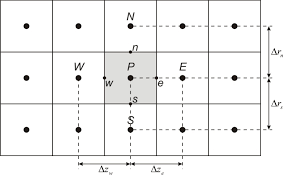
\includegraphics[width=60mm]{Imagens/malha.png}
	\caption{Exemplo de uma malha não adaptativa}
\end{figure}